%************************************************
\chapter{Evaluation}\label{ch:evaluation}
%************************************************
This chapter evaluates the three waste algorithms, as proposed in \autoref{sec:approaches}. This evaluation is based on their complexity and accuracy. Furthermore, the demo application is evaluated in \autoref{sec:demo_eval}.


\section{Optimal approach} \label{sec:optimal_approach}
In this section, three approaches from \autoref{sec:approaches} are evaluated using their complexity and accuracy. 

\subsection{Complexity}
The complexity can be expressed in terms of memory complexity and computational complexity. They are all listed in \autoref{tab:complexity}. The minimal complexity for both memory and computational is $\mathcal{O}(n)$, as a host runs $n$ containers. Approach 2 has a memory complexity of $\mathcal{O}(n)$ as this algorithm only iterates the utilization values as well. Approach 3 has a computational complexity of $\mathcal{O}(n^3)$ as this is necessary for solving a system of linear equations in the worst case. However, \cite{pan1991complexity} explains that there exists several optimization and thus may be usually be done in $\mathcal{O}(n^2)$.\\

\noindent
As approach \ref{sec:proportional} is clearly the worst in terms of memory and computational complexity it can be argued that $n$ is usually not a very large number, as it represents the number of containers for a specific host. According to a survey from 2017 \cite{docker_report}, the median number of containers per host is 10. However, this survey also stated that they have a response with 95 containers per host. In both cases, the waste can be easily computed. On an average machine, computing the waste for for $n = 100$ takes less than 1 millisecond. Given that this needs to be computed only once an hour, all three approaches are sufficient.

\begin{table}[ht]
    \centering
    \begin{tabular}{l|c|c}
        \textbf{Approach} & \textbf{Memory} & \textbf{Computational} \\ \hline
        \ref{sec:equal} & $\mathcal{O}(n)$ & $\mathcal{O}(n)$ \\
        \ref{sec:linear} & $\mathcal{O}(n)$ & $\mathcal{O}(n \log n)$ \\
        \ref{sec:proportional} & $\mathcal{O}(n^2)$ & $\mathcal{O}(n^3)$ \\
    \end{tabular}
    \caption{Memory and Computational complexity for the three different approaches}
    \label{tab:complexity}
\end{table}

\subsection{Accuracy} \label{sec:data}
As the previous section has shown that the computational and memory complexity is not significant in choosing the best approach, it is interesting to investigate the difference in their results. This section shows the actual values and whether these can be justified. In order to do so, several utilization distributions have been generated and have been listed in \autoref{tab:values}. This table provides two examples with $n = 2$, and two examples with $n = 3$. In the first row, the waste for all three approaches are approximately equivalent. However, in the second row, the waste varies a lot between the different approaches. It doesn't feel natural that, if a container utilizes 4 times more than another container, its corresponding waste is the same. Therefore, the computations from the approach described in \autoref{sec:equal} feel to simplistic.\\

\noindent
In the case of $n = 3$, the table provides two examples. It can be observed that the approach describes in \autoref{sec:linear} returns $0$ if the utilization is too high. However, this might also feel unnatural, as there is the notion that every container might be able to reduce its waste. It also needs to be stated that the approach from \autoref{sec:proportional} might seem incorrect as well, as the it is based on the assumption that every container utilizes and wastes the same amount ($u_i * w_i = c$). Although it is required that $u_i > 0$, it can be close to $0$. This leads to the fact that this container utilizes almost every waste, i.e. $w_i \approx \sum_{i=1}^n w_i$.\\

\noindent
Apart from presenting the data in a table, it is also possible to visualize this in a graph. This visualization can be found in Figure \ref{fig:approaches}. It consists of two examples of utilization distributions, each consisting of two utilization values. This visualization should be interpreted by drawing a vertical line from the utilization values to the waste values. For example, in \autoref{fig:approaches:A}, the utilization values in the left most position are $u_1 = 0.2$ and $u_2 = 0$. This results in $w_1 = w_2 = 0.4$ for approach 1, $w_1 = 0.3, w_2 = 0.5$ for approach 2, and $w_1 = 0, w_2 = 0.8$ for approach 3. Using \autoref{fig:approaches:A}, it can be observed how the waste values change if one utilization value remains constant, while the other utilization value increases. In \autoref{fig:approaches:B} it can be observed how the waste values change while one utilization value increases and another decreases. In this figure, the sum of the utilization values remains constant, while it increases in \autoref{fig:approaches:A}.

\begin{table}
    \centering
    \begin{tabular}{|r|r|r|r|c|r|r|r|r|}
        \hline
        \multicolumn{4}{|c|}{\textbf{Utilization}} & \multirow{2}{*}{\textbf{Approach}} & \multicolumn{4}{|c|}{\textbf{Waste}} \\ 
        $u_1$ & $u_2$ & $u_3$ & $\sum$ & \multirow{2}{*}{} & $w_1$ & $w_2$ & $w_3$ & $\sum$ \\ \hline
        
        \multirow{3}{*}{0.10} & \multirow{3}{*}{0.15} &  & \multirow{3}{*}{0.25} 
        & \ref{sec:equal} & 0.375 & 0.375 & &                            \multirow{3}{*}{0.75} \\
        \multirow{3}{*}{}     & \multirow{3}{*}{}     & & \multirow{3}{*}{}
        & \ref{sec:linear} & 0.4 & 0.35 & & \multirow{3}{*}{} \\
        \multirow{3}{*}{}     & \multirow{3}{*}{}     & & \multirow{3}{*}{}
        & \ref{sec:proportional} & 0.45 & 0.3 & & \multirow{3}{*}{} \\ \hline
        
        \multirow{3}{*}{0.60} & \multirow{3}{*}{0.15} &  & \multirow{3}{*}{0.75} 
        & \ref{sec:equal} & 0.125 & 0.125 & &                            \multirow{3}{*}{0.25} \\
        \multirow{3}{*}{}     & \multirow{3}{*}{}     & & \multirow{3}{*}{}
        & \ref{sec:linear} & 0 & 0.25 & & \multirow{3}{*}{} \\
        \multirow{3}{*}{}     & \multirow{3}{*}{}     & & \multirow{3}{*}{}
        & \ref{sec:proportional} & 0.05 & 0.20 & & \multirow{3}{*}{} \\ \hline
        
        \multirow{3}{*}{0.10} & \multirow{3}{*}{0.35} & \multirow{3}{*}{0.35} & \multirow{3}{*}{0.80} 
        & \ref{sec:equal} & 0.067 & 0.067 & 0.067 & \multirow{3}{*}{0.20} \\
        \multirow{3}{*}{}     & \multirow{3}{*}{}     & \multirow{3}{*}{} & \multirow{3}{*}{}
        & \ref{sec:linear} & 0.20 & 0 & 0 & \multirow{3}{*}{} \\
        \multirow{3}{*}{}     & \multirow{3}{*}{}     & \multirow{3}{*}{} & \multirow{3}{*}{}
        & \ref{sec:proportional} & 0.127 & 0.036 & 0.036 & \multirow{3}{*}{} \\ \hline
        
        \multirow{3}{*}{0.05} & \multirow{3}{*}{0.05} & \multirow{3}{*}{0.45} & \multirow{3}{*}{0.55} 
        & \ref{sec:equal} & 0.15 & 0.15 & 0.15 & \multirow{3}{*}{0.45} \\
        \multirow{3}{*}{}     & \multirow{3}{*}{}     & \multirow{3}{*}{} & \multirow{3}{*}{}
        & \ref{sec:linear} & 0.225 & 0.225 & 0 & \multirow{3}{*}{} \\
        \multirow{3}{*}{}     & \multirow{3}{*}{}     & \multirow{3}{*}{} & \multirow{3}{*}{}
        & \ref{sec:proportional} & 0.213 & 0.213 & 0.023 & \multirow{3}{*}{} \\ \hline
        
    \end{tabular}
    \caption{Several utilization values and the waste values that are computed using the three approaches}
    \label{tab:values}
\end{table}


\begin{figure}
    \subfloat[Example 1]{%
        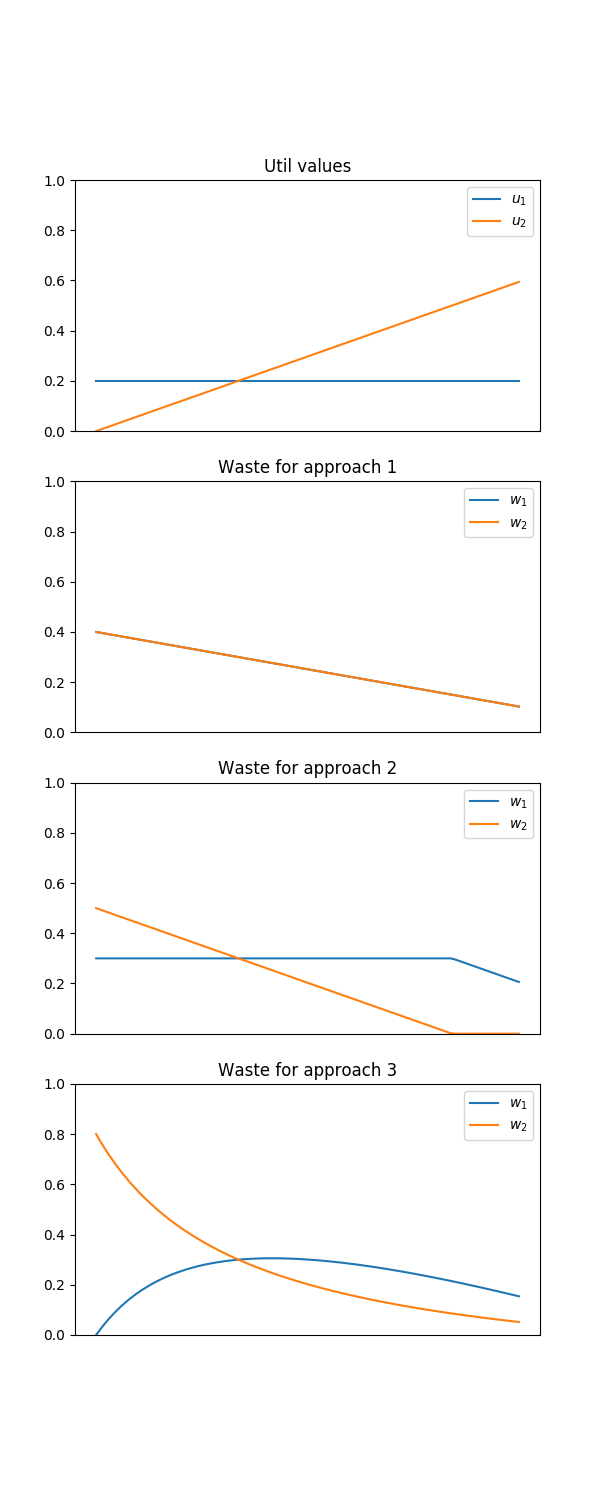
\includegraphics[width=6cm]{gfx/exampleA.png}%
        \label{fig:approaches:A}%
    }\qquad
    \subfloat[Example 2]{%
        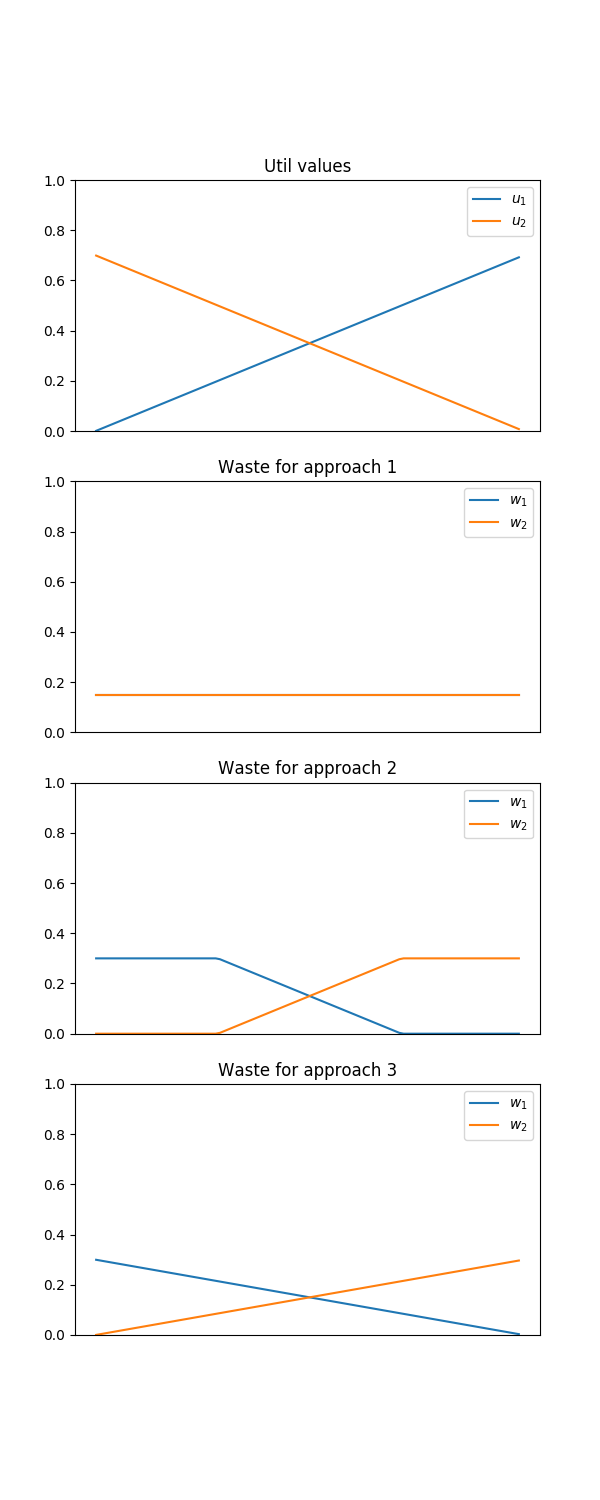
\includegraphics[width=6cm]{gfx/exampleB.png}%
        \label{fig:approaches:B}%
    }
    \caption{Two utilization values and their corresponding waste distribution}
    \label{fig:approaches}
\end{figure}


\subsection{Conclusion} \label{sec:conclusion4}
One of the properties of the utilization values (as stated in \autoref{sec:waste_requirements}) is that $u_i > 0$ for all $i$. However, while deploying the system, it turned out that the utilization of a certain container was zero. In the first two approaches (\autoref{sec:equal} and \autoref{sec:linear}), this is not a problem. However, this is a problem for the last approach (\autoref{sec:proportional}). An example can be seen for $n = 3$ with $u_1 = 0.3, u_2 = 0, u_3 = 0.2$. This results in the waste values: $w_1 = 0, w_2 = 0.5, w_3 = 0$. Therefore, if $u_1 = 0$, then $w_i = 1 - u$.\\

\noindent
In case there are two containers that have a zero utilization, than the waste cannot be computed for the third approach. This is due to the fact that the matrix $A_n$ does not have a full rank anymore (as two rows are the same). This problem can be avoided by adding a small utilization value $\Delta$ to the $u_i$-values that are $0$. This value can then be removed from the corresponding $w_i$ value, to ensure that property 1 still holds. However, as explained in \autoref{sec:data}, the corresponding $w_i$ will be close to $\sum_{j=1}^n w_j$ and will lead to abnormal results. This leads to the conclusion that only the approach from \autoref{sec:linear} is sufficient for the implementation. Thus, Algorithm \ref{alg:linear} will be used to compute the waste values given the utilization values.


\section{Demo app evaluation} \label{sec:demo_eval}

\section{Internet traffic accuracy evaluation} \label{sec:eval_k}
This section provides a small research about the accuracy of the internet traffic monitoring. In order to do so, a supernode was deployed to monitor two local containers. One container acting as a web-service, and one container continuously sending requests. The command for deploying the supernode can be found in \autoref{sec:deploy_supernode}. The other two containers are deployed using the following command:

\begin{lstlisting}[language=bash, caption=Docker-compose]
curl -sS https://raw.githubusercontent.com/dadvisor/docker-compose/master/docker-compose.yml > docker-compose.yml
docker-compose up -d 
\end{lstlisting}

\noindent
The idea behind evaluating the accuracy is to allow only one container to communicate with the web-service. By doing so, the total amount of data that a container sends is equivalent to its internal amount of data. Thus, the following variables should hold the same value:
\begin{itemize}
    \item \textbf{network\_container\_total}: This metric receives a value by scraping data from cAdvisor.
    \item \textbf{bytes\_send\_total}: This metrics has a key-value pair with both `src' and `dst'. This is the amount of data sent between the source container and the destination container by reading the Tcpdump data.
\end{itemize}

\noindent
By analysing the rate (per-second average rate of increase) over a time period of one hour, the accuracy can be determined. This can be expressed as the ratio between the two variables above. A perfect estimation would therefore result in a value of 1. The Prometheus query for analysing the accuracy is presented below.

\begin{verbatim}
rate(network_container_total[5m]) / on (src) 
rate(bytes_send_total[5m])
\end{verbatim}

\noindent
Several analyses have been made for different K values, as proposed in \autoref{sec:decisions}. Apart from the K value, the average CPU usage of the supernode is also measured. The results can be found in \autoref{tab:accuracy_results}. The data obtained for $K = 9$ can be found in \autoref{fig:network_traffic_accuracy}. In this figure, the web-service is presented in green, while the request-service is denoted in yellow.

\begin{figure}
    \centering
    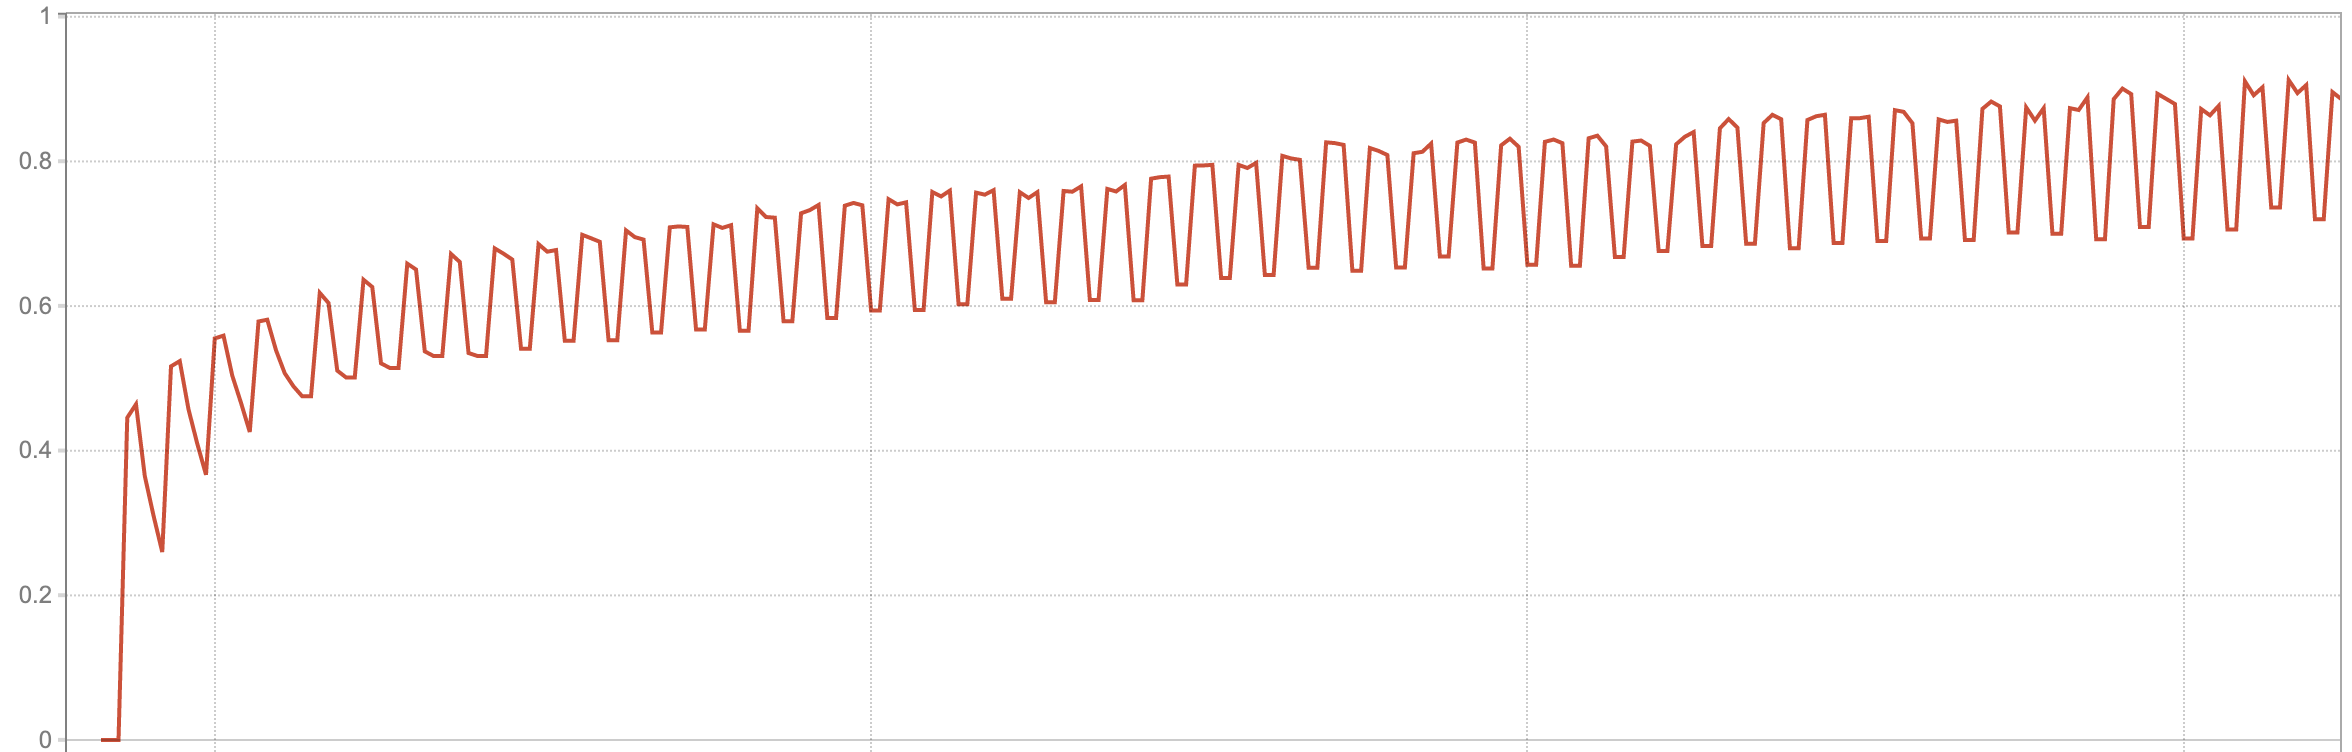
\includegraphics[width=\textwidth]{gfx/traffic_network_accuracy}
    \caption{Network traffic accuracy}
    \label{fig:network_traffic_accuracy}
\end{figure}

\begin{table}[ht]
    \centering
    \begin{tabular}{r|rrr}
        K-value & minimum accuracy & maximum accuracy & CPU usage \\ \hline
        9 & 2.7 & 3.3 & 2.2\% \\
        
    \end{tabular}
    \caption{Network traffic accuracy results for different K-values}
    \label{tab:accuracy_results}
\end{table}

